\section{Methodology \& Implementation} 

\begin{frame}[label=methodologyimplementation]{Methodology and Implementation}

\begin{block}{Objective}
    \begin{itemize}
        \item Forecast next-day WDAY stock prices using LSTM and LSTM-BiGRU models
        \item Assess robustness in volatile, mid-cap stock environments
    \end{itemize}
\end{block}

\note{
We now present both the methodological framework and its practical implementation, covering data 
preparation, model building, and evaluation.
}
\end{frame}


\begin{frame}[label=timeline, shrink]{Project Timeline: From Data to Prediction}

\begin{center}
\centerresizebox{
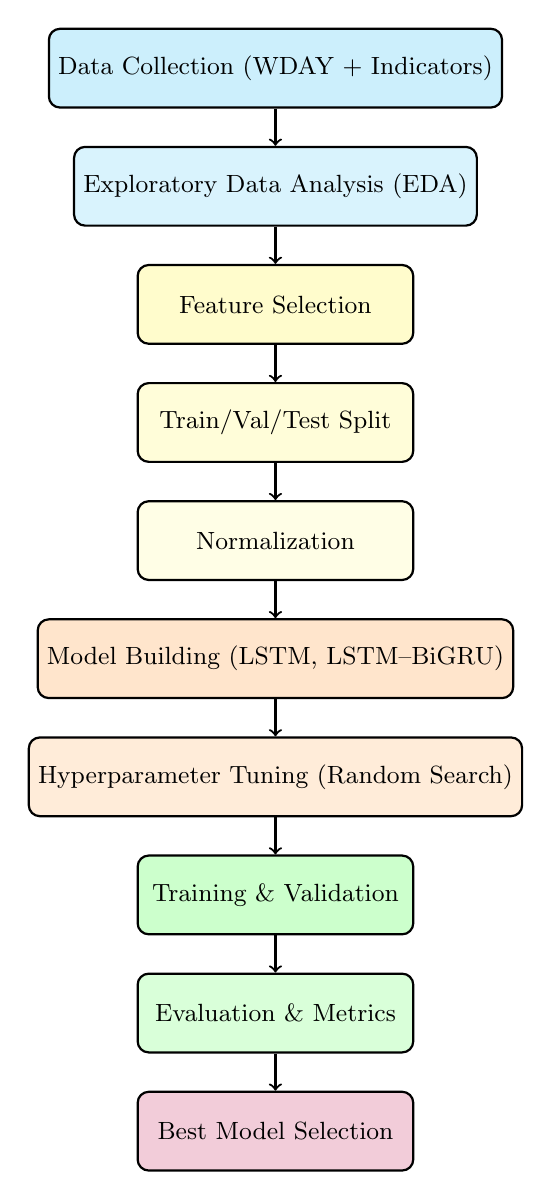
\begin{tikzpicture}[node distance=1.5cm, every node/.style={draw, rectangle, rounded corners, minimum width=3.5cm, minimum height=1cm, font=\small, align=center}, every path/.style={draw, thick, ->}]

% Nodes
\node[fill=cyan!20]  (start) {Data Collection (WDAY + Indicators)};
\node[fill=cyan!15] (eda) [below of=start] {Exploratory Data Analysis (EDA)};
\node[fill=yellow!20] (feature) [below of=eda] {Feature Selection};
\node[fill=yellow!15] (split) [below of=feature] {Train/Val/Test Split};
\node[fill=yellow!10] (normalization) [below of=split] {Normalization};
\node[fill=orange!20] (build) [below of=normalization] {Model Building (LSTM, LSTM–BiGRU)};
\node[fill=orange!15] (tuning) [below of=build] {Hyperparameter Tuning (Random Search)};
\node[fill=green!20] (train) [below of=tuning] {Training \& Validation};
\node[fill=green!15] (evaluation) [below of=train] {Evaluation \& Metrics};
\node[fill=purple!20] (end) [below of=evaluation] {Best Model Selection};

% Arrows
\draw (start) -- (eda);
\draw (eda) -- (feature);
\draw (feature) -- (split);
\draw (split) -- (normalization);
\draw (normalization) -- (build);
\draw (build) -- (tuning);
\draw (tuning) -- (train);
\draw (train) -- (evaluation);
\draw (evaluation) -- (end);

\end{tikzpicture}
}
\end{center}

\note{
This diagram outlines the full deep learning pipeline used to predict Workday’s stock price.

We begin with data collection, which includes WDAY historical prices and technical indicators like moving averages and RSI. Next, we perform exploratory data analysis to understand trends, patterns, and data quality.

Feature selection reduces noise by retaining only the most relevant inputs. The dataset is then split chronologically into training, validation, and test sets, and normalized to ensure stable input ranges for LSTM models.

Model building involves creating both LSTM and LSTM–BiGRU architectures, which are capable of capturing temporal dependencies. We tune hyperparameters like layer size, learning rate, and dropout using random search to optimize performance.

The best model is trained and validated, and evaluated on the test set using metrics like MAE and RMSE. Finally, the most robust and generalizable model is selected for analysis.

This structured process ensures the models are both well-tuned and realistically tested under conditions of volatility and limited data.
}
\end{frame}

\begin{frame}[label=datacollectioneda]{Data Collection and Initial Analysis}

\begin{block}{Sources}
    \begin{itemize}
        \item WDAY stock data via Twelve Stock Market API
        \item 10 years of daily OHLCV prices (2014–2025)
        \item Technical indicators for trend, momentum, volatility, and volume
    \end{itemize}
\end{block}

\begin{alertblock}{Exploratory Data Analysis (EDA)}
    2,820 clean daily records analyzed for descriptive statistics and volatility behavior (a decent but relatively small dataset by deep learning standards).
\end{alertblock}

\note{
We collected 10 years of daily WDAY data, enabling a robust view of long-term economic cycles.
Technical indicators were calculated, offering momentum, trend, and volatility insights.
The EDA showed that the dataset was clean and stable, providing a strong basis for modeling.
}
\end{frame}

\begin{frame}[label=datastructure,shrink]{Dataset Overview: Features and Indicators}
\begin{table}
\centering
\caption{Categories of Features in the WDAY Dataset}
\label{tab:datasetstructure}
\renewcommand{\arraystretch}{1.7} 
\begin{tabular}{p{2cm}p{12.5cm}}
\hline
\textbf{Category} & \textbf{Description} \\
\hline\hline
\textbf{Pricing} & Includes daily Open, High, Low, Close, and Volume (OHLCV) 
values, serving as the \alert{foundation for tracking stock performance}. \\
\textbf{Trend} & Measure the overall market direction, 
\alert{helping to identify uptrends, downtrends}, or sideways movements. \textit{Example: Moving Average Convergence Divergence (MACD)}. \\
\textbf{Momentum} & Evaluate the \alert{speed and strength of price movements},
providing insights into potential trend reversals and overbought/oversold 
conditions. \textit{Example: Relative Strength Index (RSI)}. \\
\textbf{Volatility} & Assess market risk and \alert{price fluctuations}, identifying 
potential breakouts and periods of stability. {\textit{Example: Bollinger Bands Width}.} \\
\textbf{Volume} & Analyze trading activity to confirm price trends and \alert{detect accumulation (buying) or distribution (selling) behavior}. \textit{Example: On-Balance Volume (OBV)}. \\
\hline
\end{tabular}
\end{table}

\note{
The dataset is structured around five major feature categories.
Pricing Data (OHLCV) forms the base, while Trend, Momentum, Volatility, and Volume indicators enrich the inputs.
These indicators offer critical signals about market behavior, improving the model's ability to forecast stock price movements.
Using multiple indicator types ensures the model captures various dimensions of stock performance, not just raw prices.
}
\end{frame}

\begin{frame}[label=datawindow,shrink]{Why 10 Years of Daily Data?}

\small
\begin{table}
\centering
\caption{Recommended Data Windows and Interval for Stock Price Prediction}
\label{tab:data-window}
\renewcommand{\arraystretch}{1.7} 
\begin{tabular}{p{2cm}p{2cm}p{2cm}p{4cm}}
\hline
\textbf{Study} & \textbf{Window} & \textbf{Interval} & \textbf{Use Case} \\
\hline\hline
\parencite{shaban2024SMPDL} & 2 Years & Every Minute & High-frequency trading (HFT) \\
\parencite{guo2024LSTMStock} & 125 days & Every Minute & HFT bursts, micro-movement learning \\
\parencite{chang2024StockPrediction}, \parencite{nabipour2020DeepLearning} & 
\alert{10 Years} & \alert{Daily} & \alert{Medium-term forecasting} \\
\hline
\end{tabular}
\end{table}

\note{
Here’s the reasoning behind our choice:

- \textbf{Shaban et al. (2024)} used minute-level data for HFT. While very precise, it is extremely noisy, requires heavy computation, and is often unsuitable for broader trend forecasting.
- \textbf{Guo et al. (2024)} also used minute data but only over short bursts (125 days). Again, good for micro-movement analysis, but lacks the ability to capture economic cycles or mid-term patterns.
- \textbf{Chang (2024)} and \textbf{Nabipour (2020)} chose 10 years of daily data. This approach captures complete economic cycles, offers broader trend detection, and aligns better with end-of-day price prediction goals.

Thus, our methodology adopts a daily, 10-year window to focus on generalizable, meaningful stock trends rather than short-term noise.
}
\end{frame}

\begin{frame}[label=datasetsplit, shrink]{Dataset Split Strategy}

\small

\begin{block}{Why Time-Based Splitting?}
\begin{itemize}
    \item Time-series data must maintain chronological order to avoid data leakage.
    \item Ensures that the model only uses \textbf{past} information to predict the \textbf{future}.
    \item Aligns with best practices in financial forecasting research~\parencite{chang2024StockPrediction, guo2024LSTMStock}.
\end{itemize}
\end{block}

\vspace{0.5em}
{\footnotesize
\begin{equation}
\label{eq:dataset_split_dates}
\underbrace{X_{\text{2014-01-02}}, \dots, X_{\text{2021-11-08}}}_{\text{Training Data (75\%)}} 
\quad
\underbrace{X_{\text{2021-11-09}}, \dots, X_{\text{2023-07-20}}}_{\text{Validation Data (15\%)}} 
\quad
\underbrace{X_{\text{2023-07-21}}, \dots, X_{\text{2025-03-28}}}_{\text{Test Data (15\%)}} 
\end{equation}
}
\note{
In financial forecasting, preserving the temporal structure is crucial.

We split the dataset chronologically:
\begin{itemize}
    \item 75\% for training — covering over 7 years of historical patterns.
    \item 15\% for validation — tuning hyperparameters.
    \item 15\% for testing — strictly future, unseen data from volatile periods.
\end{itemize}
The chronological split avoids any future data leakage into training and reflects real-world stock prediction challenges.
}
\end{frame}

\begin{frame}[label=featurescalingworkflow]{Feature Scaling Workflow: How We Prevent Leakage}

\small

\begin{block}{Scaler Fitting and Application}
\begin{itemize}
    \item \textbf{MinMaxScaler} is \textbf{fit only on the Training Set}.
    \item The learned scaling parameters ($x_{\min}$, $x_{\max}$) are reused for Validation and Test Sets.
    \item Ensures consistent input distribution and prevents leakage.
\end{itemize}
\end{block}

\begin{alertblock}{Why MinMaxScaler for LSTM?}
MinMaxScaler ensures that inputs match LSTM activation functions (tanh/sigmoid), improving training stability, convergence speed, and balancing feature influence
~\parencite{shaban2024SMPDL,phuoc2024StockPrediction}.
\end{alertblock}

\note{
In financial time-series forecasting, it is essential to avoid data leakage when scaling features.

We fit the MinMaxScaler exclusively on the Training Set. 
This ensures that the scaler parameters are only influenced by past information.
Then, we reuse these parameters when scaling the Validation and Test sets.

This approach mirrors a real-world scenario where future data is unknown during model training, ensuring that model performance evaluation is realistic and unbiased.
}
\end{frame}

\begin{frame}[label=lstm_architecture]{Model Architecture -- Layered LSTM}

\begin{columns}[c] % center vertically aligned
    \begin{column}{0.7\textwidth}
        \begin{block}{Overview}
            \begin{itemize}
                \item Two stacked LSTM layers to capture long-term sequential patterns.
                \item Dropout layers after each LSTM to prevent overfitting.
                \item Dense output layer to predict the next day's closing price.
                \item Simple yet powerful model for financial time-series forecasting.
            \end{itemize}
        \end{block}
    \end{column}
    
    \begin{column}{0.28\textwidth}
        \centering
        \resizebox{0.7\textwidth}{!}{
        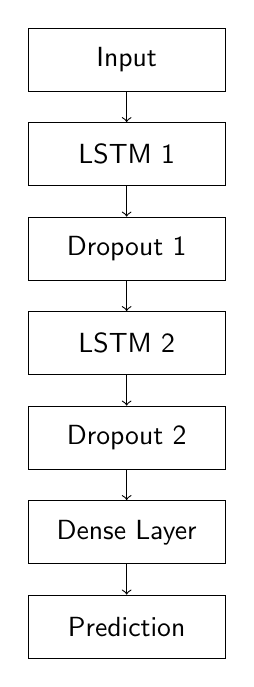
\begin{tikzpicture}[node distance=1.2cm, every node/.style={draw, minimum width=2.5cm, minimum height=0.8cm, font=\sffamily, align=center}]
            \node(input) {Input};
            \node[below of=input] (lstm1) {LSTM 1};
            \node[below of=lstm1] (drop1) {Dropout 1};
            \node[below of=drop1] (lstm2) {LSTM 2};
            \node[below of=lstm2] (drop2) {Dropout 2};
            \node[below of=drop2] (dense) {Dense Layer};
            \node[below of=dense] (output) {Prediction};
            \draw[->] (input) -- (lstm1);
            \draw[->] (lstm1) -- (drop1);
            \draw[->] (drop1) -- (lstm2);
            \draw[->] (lstm2) -- (drop2);
            \draw[->] (drop2) -- (dense);
            \draw[->] (dense) -- (output);
        \end{tikzpicture}
        }
    \end{column}
\end{columns}

\note{
The LSTM architecture uses two LSTM layers to model long-term temporal dependencies,
followed by dropout layers to regularize the model and prevent overfitting.
Finally, a Dense layer maps the learned representations into a next-day price prediction.
This simple but robust design is commonly used in stock forecasting tasks.

Just as adding exponents or higher-order terms makes a mathematical function more flexible and expressive, stacking LSTM or BiGRU layers enhances the model’s ability to learn complex, long-term patterns in sequential stock price data.
}
\end{frame}


\begin{frame}[label=lstmbigru_architecture]{Model Architecture -- Hybrid LSTM-BiGRU}

\begin{columns}[c]
    \begin{column}{0.7\textwidth}
        \begin{block}{Overview}
            \begin{itemize}
                \item BiGRU layer captures both past and future dependencies.
                \item Followed by 3 stacked LSTM layers for sequence refinement.
                \item Dropout layers prevent overfitting at each stage.
                \item Dense layer outputs the next-day stock price.
            \end{itemize}
        \end{block}
    \end{column}
    
    \begin{column}{0.28\textwidth}
        \resizebox{0.45\textwidth}{!}{
        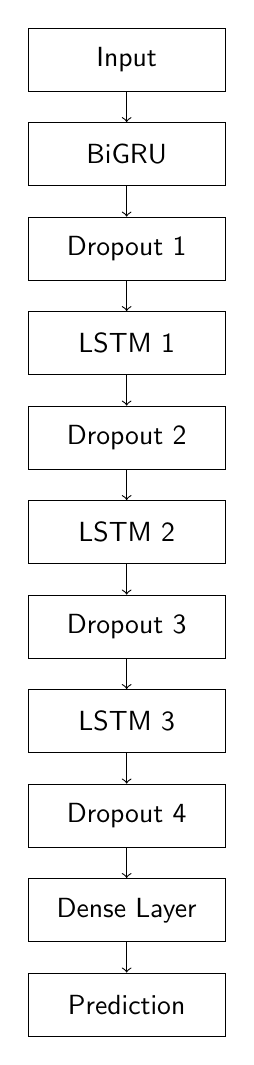
\begin{tikzpicture}[node distance=1.2cm, every node/.style={draw, minimum width=2.5cm, minimum height=0.8cm, font=\sffamily, align=center}]
            \node(input) {Input};
            \node[below of=input] (bigru) {BiGRU};
            \node[below of=bigru] (drop1) {Dropout 1};
            \node[below of=drop1] (lstm1) {LSTM 1};
            \node[below of=lstm1] (drop2) {Dropout 2};
            \node[below of=drop2] (lstm2) {LSTM 2};
            \node[below of=lstm2] (drop3) {Dropout 3};
            \node[below of=drop3] (lstm3) {LSTM 3};
            \node[below of=lstm3] (drop4) {Dropout 4};
            \node[below of=drop4] (dense) {Dense Layer};
            \node[below of=dense] (output) {Prediction};
            \draw[->] (input) -- (bigru);
            \draw[->] (bigru) -- (drop1);
            \draw[->] (drop1) -- (lstm1);
            \draw[->] (lstm1) -- (drop2);
            \draw[->] (drop2) -- (lstm2);
            \draw[->] (lstm2) -- (drop3);
            \draw[->] (drop3) -- (lstm3);
            \draw[->] (lstm3) -- (drop4);
            \draw[->] (drop4) -- (dense);
            \draw[->] (dense) -- (output);
        \end{tikzpicture}
        }
    \end{column}
\end{columns}

\note{
The LSTM-BiGRU hybrid architecture first uses a BiGRU to capture sequential information from both directions.
Then, three LSTM layers refine the learned patterns, allowing the model to better detect future stock trends.
Dropouts help prevent overfitting, while the final Dense layer generates the next-day price prediction.
}
\end{frame}

\begin{frame}[label=regularization, shrink]{Preventing Overfitting and Underfitting}

\begin{block}{Key Regularization Techniques}
    \begin{itemize}
        \item \textbf{Adam Optimizer:} Adaptive learning rate that helps reach optimal weights faster and avoids poor local minima.
        \item \textbf{Dropout Layers:} Randomly deactivate neurons during training to prevent co-adaptation and reduce overfitting.
        \item \textbf{Early Stopping:} Monitors validation loss and stops training once performance stops improving, preventing overfitting on the training data.
    \end{itemize}
\end{block}

\begin{alertblock}{Goal}
    These techniques work together to balance model complexity and generalization, ensuring the model learns meaningful patterns without memorizing noise.
\end{alertblock}

\note{
To avoid overfitting (memorizing noise) or underfitting (missing real patterns), we use several strategies.
Adam helps find better solutions faster with dynamic learning rates.
Dropout forces the model to learn redundant paths, preventing over-dependence.
Early stopping saves the best version of the model before overfitting starts on validation data.
Together, they create a more reliable and generalizable predictor.
}
\end{frame}

\begin{frame}[label=hyperparamtuning, shrink]{Hyperparameter Tuning Strategy}
\begin{block}{Why Random Search?}
\begin{itemize}
    \item \textbf{Grid Search} tests every possible combination exhaustively. 
    It is \alert{extremely time-consuming in high dimensions}.
    \item \textbf{Random Search} samples combinations randomly, \alert{covering the
    space more efficiently and often finding good models faster}.
\end{itemize}
\end{block}

\begin{exampleblock}{Implementation Details}
\begin{itemize}
    \item Random Search was implemented using \texttt{KerasTuner} from the TensorFlow Keras API.
    \item It optimized key parameters such as learning rate, hidden units, dropout rate, and sequence length.
\end{itemize}
\end{exampleblock}

\note{
Grid Search becomes computationally infeasible as the number of hyperparameters grows.
Random Search provides a practical alternative by efficiently exploring the parameter space.
It is especially useful when many hyperparameters have little effect and only a few are critical.
KerasTuner's RandomSearch was used to implement this process.
}
\end{frame}

\begin{frame}[label=hyperparamconfig, shrink]{Hyperparameter Search Space}
\centering
\begin{table}[h]
\renewcommand{\arraystretch}{1.7} 

\begin{tabular}{p{3cm}p{3.5cm}p{6.5cm}}
\hline
\textbf{Hyperparameter} & \textbf{Values Range} & \textbf{Purpose} \\
\hline\hline
Learning Rate & 0.0001 – 0.001 & Fine-tunes convergence speed~\parencite{parmar2018stock}.\\
Hidden Units & 16, 32, 64, 128 & Balances capacity and overfitting risk.\\
Dense Units & 16, 32 & Size of final prediction layer.\\
Dropout Rate & \alert{0.01}, 0.2, 0.3 & Random deactivation to prevent overfitting~\parencite{agrawal2022StockPrediction}.\\
Sequence Length & 30 – 90 & Window of historical time steps considered.\\
Batch Size & 64 & Training stability and memory efficiency.\\
Epochs & 200 & Maximum training rounds.\\
Early Stopping & Patience = 10, min\_delta = $1e^{-6}$ & Halts training if no significant improvement is detected.\\
Optimizer & Adam & Adaptive optimization algorithms for RNNs.\\
\hline
\end{tabular}
\end{table}

\note{
The search explored different configurations mainly in terms of learning rate, number of hidden units, dropout levels, and sequence window size.
Random Search is statistically proven to find near-optimal hyperparameters faster in high-dimensional spaces compared to Grid Search.
}
\end{frame}

\begin{frame}[label=final_models]{Final Model Architectures and Parameters}

\begin{columns}[c]
\column{0.48\textwidth}
\textbf{LSTM Model:}
\vspace{0.3em}
\begin{table}[H]
\centering
\resizebox{\linewidth}{!}{
\begin{tabular}{lp{2.8cm}}
\hline
\textbf{Parameter} & \textbf{Value} \\
\hline\hline
Sequence Length & 30 \\
Hidden Units & LSTM$_1$: 128, LSTM$_2$: 32 \\
Dropout Rates & 0.01 after each LSTM layer \\
Dense Layer & 32 units \\
Learning Rate & 0.001 \\
Total Parameters & 292,421 \\
Trainable Parameters & 97,473 \\
\hline
\end{tabular}
}
\end{table}

\column{0.48\textwidth}
\textbf{LSTM-BiGRU Model:}
\vspace{0.3em}
\begin{table}[H]
\centering
\resizebox{\linewidth}{!}{
\begin{tabular}{lp{2.8cm}}
\hline
\textbf{Parameter} & \textbf{Value} \\
\hline\hline
Sequence Length & 30 \\
Hidden Units & BiGRU: 64, LSTM$_1$: 64, LSTM$_2$: 32, LSTM$_3$: 16 \\
Dropout Rates & BiGRU: 0.01, LSTM$_1$: 0.3, LSTM$_2$: 0.2, LSTM$_3$: 0.01
\\
Dense Layer & 16 units \\
Learning Rate & 0.001 \\
Total Parameters & 293,669 \\
Trainable Parameters & 97,889 \\
\hline
\end{tabular}
}
\end{table}

\end{columns}

\note{
This slide compares the architectural details of the LSTM and LSTM–BiGRU models used in our experiments.

Both models use a sequence length of 30, allowing them to learn from 30 prior time steps. The LSTM model features two stacked layers with 128 and 32 hidden units, and minimal regularization through a uniform dropout rate of 0.01. Its dense output layer has 32 units.

In contrast, the LSTM–BiGRU model incorporates a BiGRU layer with 64 units followed by three LSTM layers with decreasing units (64, 32, 16). This deeper structure is complemented by more aggressive and layer-specific dropout: 0.3 and 0.2 in the early LSTM layers, which helps mitigate overfitting.

Interestingly, both models maintain comparable complexity, with the LSTM–BiGRU model having just slightly more parameters—less than a 1\% increase. This means the performance gains from the hybrid model come from its structure, not its size.

This comparison supports the hypothesis that hybrid and deeper recurrent architectures may be better suited for capturing the volatility and weak signals in mid-cap stock data like Workday.

The second model outperforms the first because its deeper, hybrid architecture is better suited to capturing the non-linear and context-dependent patterns often found in volatile mid-cap stock data like Workday.
}
\end{frame}

\begin{frame}[shrink]{Performance - Training and Validation Loss Comparison}
\centering
\resizebox{1.3\linewidth}{!}{%
\begin{tabular}{m{2cm}m{10cm}}
    \textbf{LSTM} & 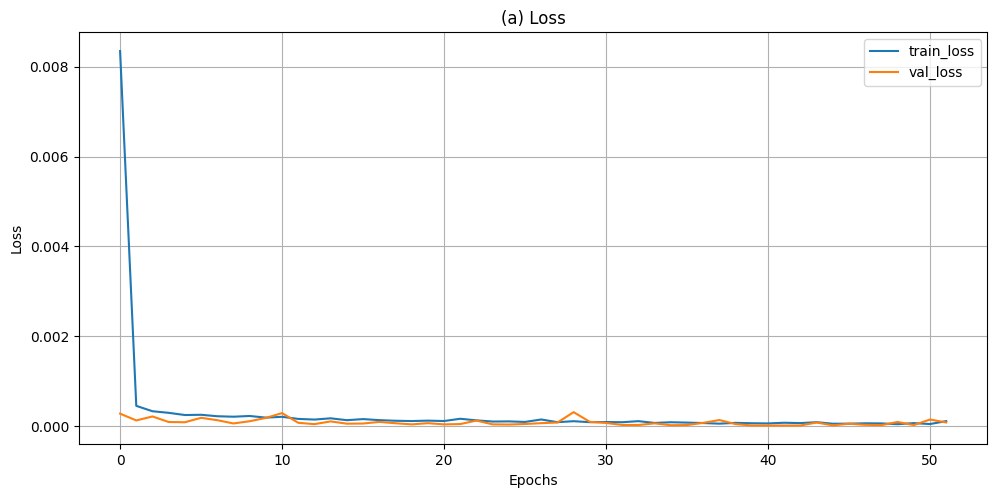
\includegraphics[width=0.7\textwidth]{img/main/lstm_loss.png} \\
    \textbf{LSTM-BiGRU} & 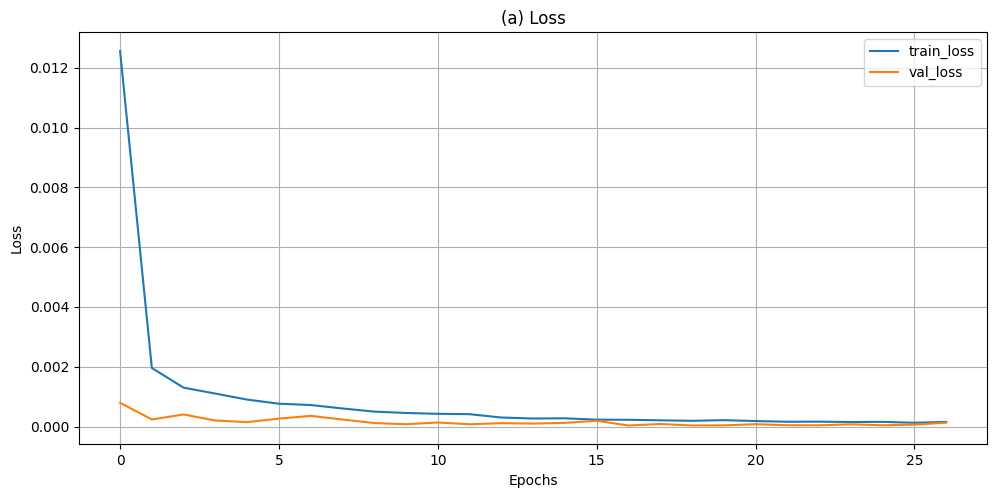
\includegraphics[width=0.7\textwidth]{img/main/bigru_loss.png} \\
\end{tabular}
}
\note{
Loss - 1Shows convergence during training (e.g., MSE or custom loss). Always 
start with Loss curves.1
Both models converge smoothly. However, the LSTM-BiGRU achieves slightly lower 
validation loss earlier, suggesting faster convergence and slightly better 
generalization.
}
\end{frame}

\begin{frame}[shrink]{Performance - Training and Validation MSE Comparison}
\centering
\resizebox{1.3\linewidth}{!}{%
\begin{tabular}{m{2cm}m{10cm}}
    \textbf{LSTM} & 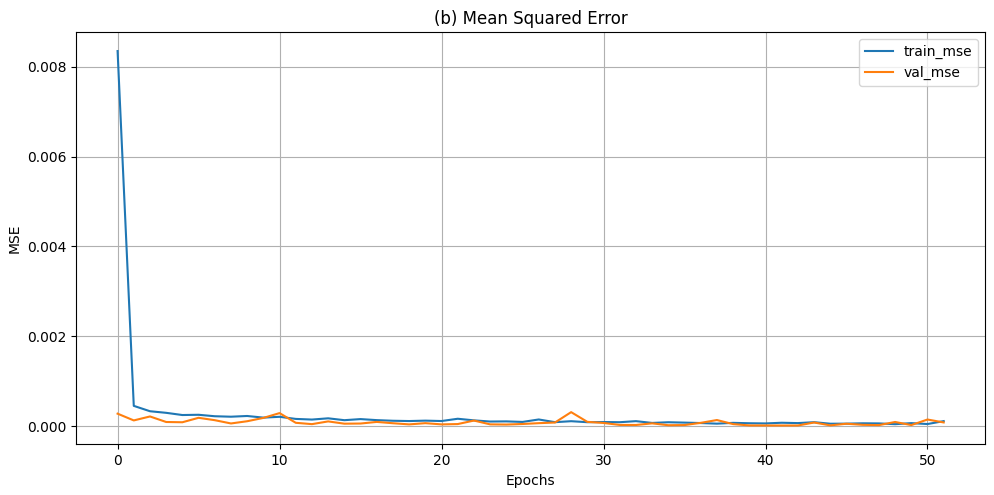
\includegraphics[width=0.7\textwidth]{img/main/lstm_mse.png} \\
    \textbf{LSTM-BiGRU} & 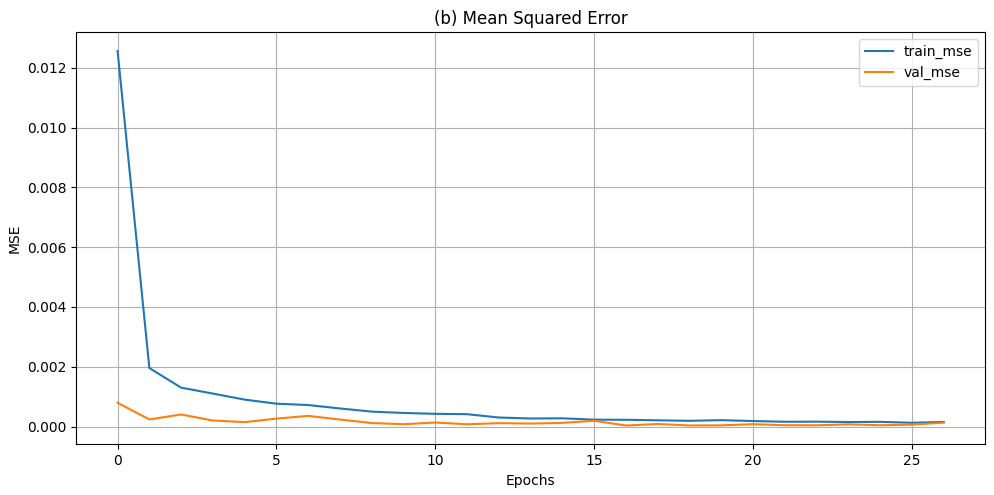
\includegraphics[width=0.7\textwidth]{img/main/bigru_mse.png} \\
\end{tabular}
}
\note{
MSE (Mean Squared Error)	Penalizes larger errors heavily (squares them),
closely tied to loss function for regression models.

Both models show a decreasing MSE trend. LSTM-BiGRU achieves lower final validation MSE, suggesting better prediction accuracy overall.
}
\end{frame}

\begin{frame}[shrink]{Performance - Training and Validation MAE Comparison}
\centering
\resizebox{1.3\linewidth}{!}{%
\begin{tabular}{m{2cm}m{10cm}}
    \textbf{LSTM} & 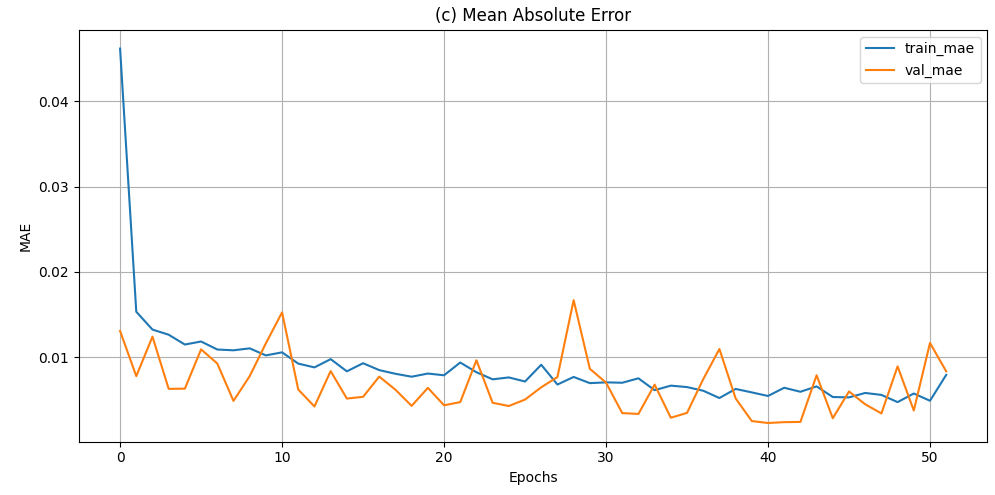
\includegraphics[width=0.7\textwidth]{img/main/lstm_mae.png} \\
    \textbf{LSTM-BiGRU} & 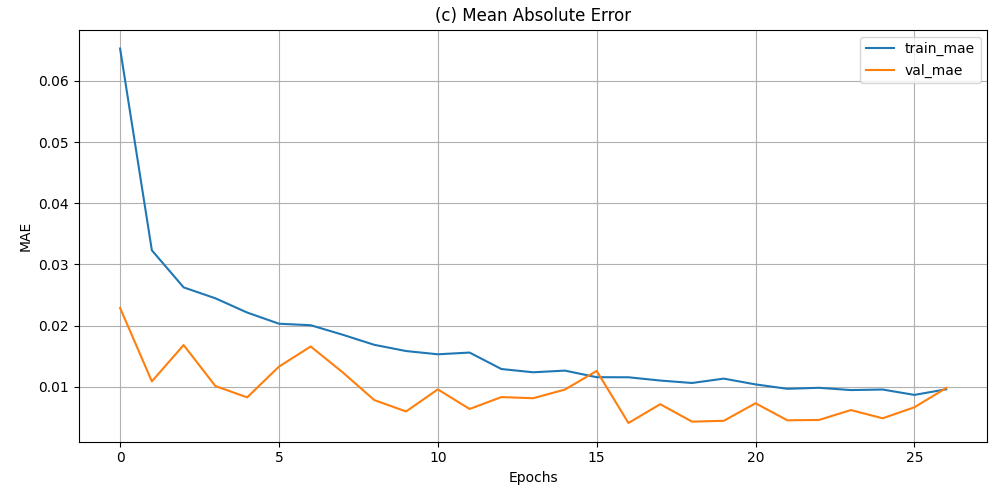
\includegraphics[width=0.7\textwidth]{img/main/bigru_mae.png} \\
\end{tabular}
}
\note{
MAE (Mean Absolute Error)	Measures average magnitude of errors without squaring, easier to interpret.

This slide compares the training and validation MAE curves for the LSTM and LSTM–BiGRU models.

The LSTM–BiGRU model achieves lower overall MAE and converges much faster—within the first 10 epochs—compared to the LSTM model, which shows slower convergence and more erratic validation error after 20 epochs. Additionally, the LSTM–BiGRU model demonstrates better generalization, with a smaller and more stable gap between training and validation errors.

This supports the conclusion that the deeper, hybrid architecture is more effective at capturing complex temporal patterns and reducing prediction error in the context of mid-cap stock data like Workday.
}
\end{frame}

\begin{frame}[shrink]{Performance - Training and Validation $R^2$ Score Comparison}
\centering
\resizebox{1.3\linewidth}{!}{%
\begin{tabular}{m{2cm}m{10cm}}
    \textbf{LSTM} & 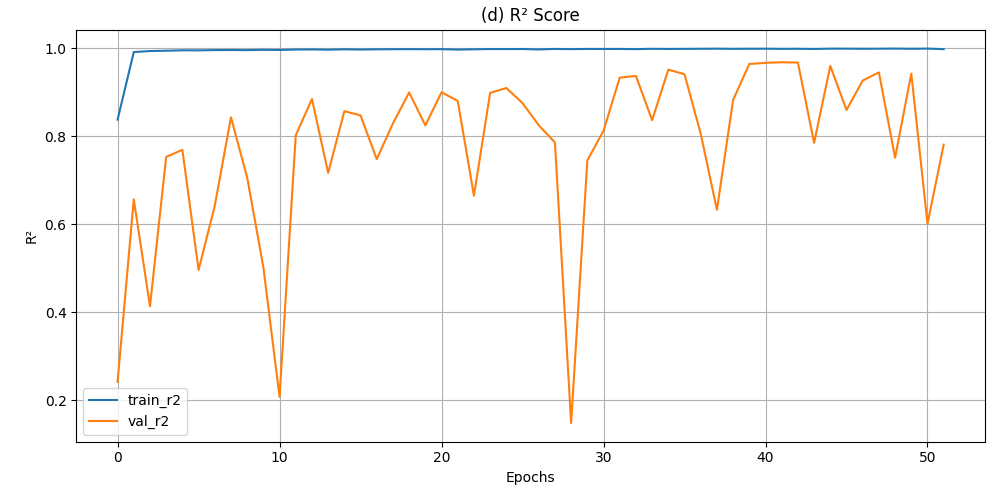
\includegraphics[width=0.7\textwidth]{img/main/lstm_r2.png} \\
    \textbf{LSTM-BiGRU} & 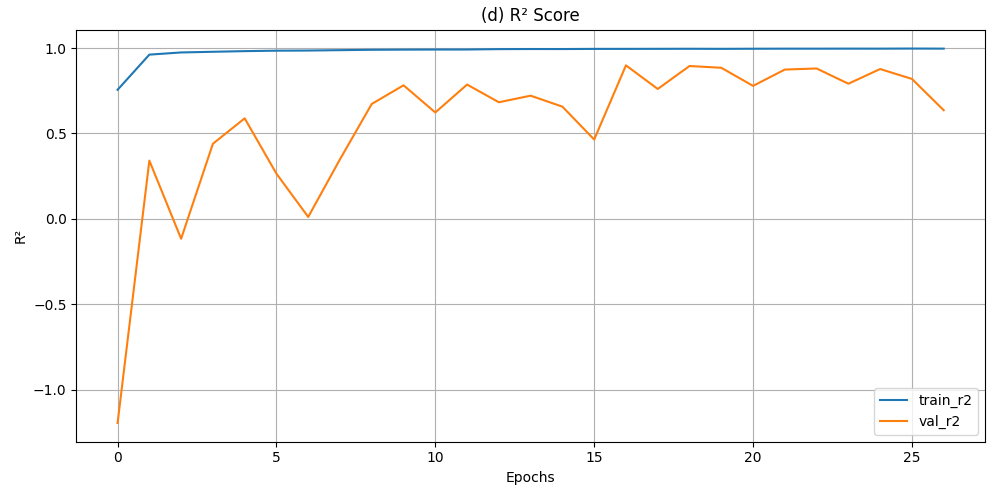
\includegraphics[width=0.7\textwidth]{img/main/bigru_r2.png} \\
\end{tabular}
}
\note{
$R^2$ Score (Coefficient of Determination)	Explains how well the model fits the data (variance explained). A summary statistic after error analysis.

Both models achieve high $R^2$ scores, but LSTM-BiGRU reaches slightly higher $R^2$ faster, indicating a better ability to explain variance in stock price movements.
}
\end{frame}

